\chapter{МАТЕМАТИЧЕСКАЯ МОДЕЛЬ ПНЕВМОПРИВОДА С ДИСКРЕТНЫМИ РАСПРЕДЕЛИТЕЛЯМИ}\label{ch:ch2}
Настоящая глава посвящена разработке математической модели пневмопривода с дискретными
распределителями как объекта управления. Для эффективного синтеза и анализа систем управления
электропневматическим приводом необходима математическая модель, учитывающая существенные
особенности объекта: нелинейную природу термодинамических процессов, переменную структуру системы при переключении
распределителей, нелинейные эффекты трения и реакцию упоров.

Особое внимание в представленном исследовании уделяется комплексному подходу к моделированию. Разработанная
математическая модель объединяет термодинамические и механические аспекты функционирования пневмопривода в
единую систему дифференциальных уравнений, описывающую динамику позиционирования с учетом всех значимых факторов.

В первом разделе главы представлена разработка математической модели позиционного пневмопривода с дискретными
распределителями, включающая модели пневмоцилиндра и распределителей, а также их интеграцию в единую систему.
Второй раздел посвящен программной реализации полученной модели и методике численного моделирования. В третьем
разделе проводится детальный анализ динамических характеристик пневмопривода с использованием метода фазовых портретов,
что позволяет выявить ключевые особенности поведения системы при различных режимах функционирования.


\section{Разработка математической модели пневмопривода с дискретными распределителями}

Исследуемый электропневматический привод представляет собой систему,
состоящую из пневматического цилиндра двустороннего действия с односторонним штоком, четырех
дискретных двухпозиционных распределителей и системы управления. Ключевой особенностью рассматриваемой
конфигурации является использование двух независимых распределителей для каждой полости цилиндра:
один служит для подачи сжатого воздуха из магистрали, другой -- для выхлопа в атмосферу. Такая схема обеспечивает
гибкое управление потоками воздуха при сохранении относительной простоты конструкции.

\begin{figure}[h]
	\centering
	\includegraphics[]{part2/actuator_calc_schemne.eps}
	\caption{Схема пневмопривода с дискретными распределителями}
	\label{fig:pneumatic_actuator}
\end{figure}

При разработке математической модели пневмопривода с дискретными распределителями приняты следующие допущения:

\begin{itemize}
	\item рабочее тело (воздух) рассматривается как идеальный газ, подчиняющийся уравнению состояния Клапейрона-Менделеева;
	\item термодинамические процессы в рабочих полостях пневмоцилиндра являются адиабатическим;
	\item температура газа в магистрали и температура окружающей среды принимаются постоянными;
	\item утечки газа через уплотнения поршня и штока не учитываются;
	\item пневматические линии между распределителями и рабочими полостями цилиндра имеют пренебрежимо малый объем по сравнению с объемом рабочих полостей;
	\item влияние сил тяжести не учитывается ввиду горизонтального расположения пневмоцилиндра.

\end{itemize}

\subsection*{Модель пневмоцилиндра}

\textbf{Уравнение движения поршня пневмоцилиндра.}
Уравнение движения пневмоцилиндра может быть получено на основе второго закона Ньютона путем
рассмотрения баланса сил, действующих на поршень в горизонтальной плоскости. Выведем данное уравнение,
последовательно учитывая все силовые факторы, оказывающие влияние на динамику системы.

На поршень действуют силы давления в полостях $R_1 = p_1F_1$ и $R_2 = p_2F_2$, атмосферного
давления $R_\text{атм} = p_\text{атм}(F_1 - F_2)$, а также сила
трения $R_\text{тр}(\dot{x})$ и реакция упоров $R_\text{упор}(x,\dot{x})$ при достижении крайних положений.
\nomenclature{$p_1, p_2$}{Давление в поршневой и штоковой полостях соответственно}
\nomenclature{$F_1, F_2$}{Эффективные площади поршня со стороны поршневой и штоковой полостей}
\nomenclature{$p_\text{атм}$}{Атмосферное давление}

Применяя второй закон Ньютона к поршню массой $M$, получаем уравнение движения:
\begin{equation}
	M\ddot{x} = p_1F_1 - p_2F_2 - p_\text{атм}(F_1 - F_2) - R_\text{тр}(\dot{x}) - R_\text{упор}(x,\dot{x}),
\end{equation}
где $x$ -- перемещение поршня; $\dot{x}$ -- скорость поршня; $\ddot{x}$ -- ускорение поршня.
\nomenclature{$x$}{Перемещение поршня}
\nomenclature{$\dot{x}$}{Скорость поршня}
\nomenclature{$\ddot{x}$}{Ускорение поршня}
\nomenclature{$M$}{Масса поршня}
\nomenclature{$R_\text{тр}(\dot{x})$}{Сила трения}
\nomenclature{$R_\text{упор}(x,\dot{x})$}{Реакция упоров}

% Эффективные площади поршня определяются его геометрическими размерами:
% $F_1 = \frac{\pi D_{\text{п}}^2}{4}$ и $F_2 = \frac{\pi(D_{\text{п}}^2 - d_{\text{шт}}^2)}{4}$,
% где $D_{\text{п}}$ -- диаметр поршня, $d_{\text{шт}}$ -- диаметр штока.
% \nomenclature{$D_{\text{п}}$}{Диаметр поршня}
% \nomenclature{$d_{\text{шт}}$}{Диаметр штока}

\textbf{Сила трения.}
В рамках математического моделирования электропневматического привода существенное значение имеет адекватное описание динамических эффектов трения,
оказывающих значительное влияние на точность позиционирования и качество переходных процессов.
Модель LuGre (Lund-Grenoble) \cite{lugre} представляет собой комплексный подход к моделированию трения,
основанный на представлении микроскопической природы контактного
взаимодействия поверхностей через концепцию щетиночной структуры.
На рисунке \ref{fig:ch2/lugre} представлена схема модели LuGre.

\begin{figure}[ht]
	\centering
	\includegraphics[]{part2/Трение.eps}
	\caption{Схема модели LuGre}
	\label{fig:ch2/lugre}
\end{figure}

Фундаментальное уравнение модели LuGre описывает эволюцию средней деформации
микронеровностей контактирующих поверхностей во времени и может быть представлено в виде дифференциального уравнения первого порядка:
\begin{equation}
	\label{eq:ch2/lugre}
	\frac{dz}{dt} = v - \frac{\sigma_0|v|}{g(v)}z,
\end{equation}
где $z$ -- средняя деформация микронеровностей;
$v$ -- относительная скорость скольжения;
$\sigma_0$ -- представляет собой коэффициент жесткости микроскопических деформаций.
\nomenclature{$z$}{Средняя деформация микронеровностей\nomrefpage}
\nomenclature{$v$}{Относительная скорость скольжения\nomrefpage}
\nomenclature{$\sigma_0$}{Коэффициент жесткости микроскопических деформаций}

Функция $g(v)$, известная как функция Штрибека, описывает характер установившегося трения и задается следующим выражением:

\begin{equation}
	\label{eq:ch2/stiction_function}
	g(v) = R_\text{к} + (R_\text{с} - R_\text{к})e^{-(|v|/v_s)^\delta},
\end{equation}
где $R_\text{к}$ -- сила кулоновского трения;
$R_\text{с}$ -- определяет силу статического трения;
$v_s$ -- характерная скорость Штрибека;
$\delta$ -- эмпирический параметр формы, для которого типичным значением считается $\delta = 2$.
\nomenclature{$v_s$}{Характерная скорость Штрибека\nomrefpage}
\nomenclature{$\delta$}{Параметр формы\nomrefpage}

Результирующая сила трения в модели LuGre формируется как суперпозиция трех составляющих:
\begin{equation}
	\label{eq:ch2/friction_force}
	R_\text{тр} = \sigma_0z + \sigma_1\dot{z} + \sigma_2v,
\end{equation}
где $\sigma_1$ -- демпфирование микродеформаций;
$\sigma_2$ -- коэффициент вязкого трения.
\nomenclature{$\sigma_1$}{Демпфирование микродеформаций\nomrefpage}
\nomenclature{$\sigma_2$}{Коеффициент вязкого трения\nomrefpage}

Для наглядной демонстрации ключевых особенностей модели LuGre на рисунке \ref{fig:lugre_characteristics} представлены графики основных характеристик трения.

\begin{figure}[ht]
	\centering
	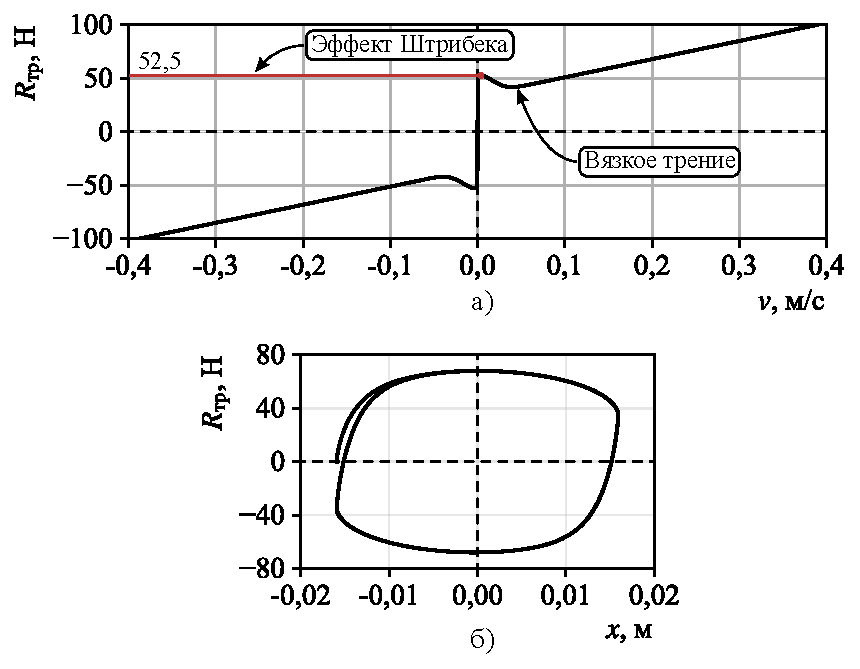
\includegraphics[]{part2/lugre_model_characteristics.pdf}
	\caption{Характеристики модели трения LuGre: а) кривая Штрибека; б) гистерезис силы трения при синусоидальном движении}
	\label{fig:lugre_characteristics}
\end{figure}

Параметры модели LuGre обладают четкой физической интерпретацией, что существенно облегчает процесс их идентификации.
Коэффициент $\sigma_0$ характеризует жесткость контактного взаимодействия микронеровностей и
определяется как предел отношения приращения силы трения к приращению деформации при стремлении последней к нулю:
\begin{equation}
	\label{eq:ch2/stiffness}
	\sigma_0 = \lim_{z \to 0} \frac{\partial R_\text{тр}}{\partial z},
\end{equation}

Параметр микродемпфирования $\sigma_1$ связан с коэффициентом жесткости через коэффициент микродемпфирования $\eta$:
\begin{equation}
	\sigma_1 = \eta\sigma_0.
\end{equation}

Коэффициент вязкого трения $\sigma_2$ определяет асимптотическое поведение силы трения при больших скоростях движения:
\begin{equation}
	\lim_{v \to \infty} \frac{R_\text{тр}}{v} = \sigma_2.
\end{equation}

В контексте электропневматического привода модель LuGre позволяет учесть ряд важных эффектов.
При малых перемещениях поршня наблюдается эффект предварительного смещения (эффект Дала), описываемый
соотношением $R_\text{пред} = \sigma_0z$ при условии $|z| < z_\text{макс}$. В области малых скоростей проявляется
нелинейная зависимость силы трения от скорости: $R_\text{нел}(v) = g(v)\text{sign}(v) + \sigma_2v$. При
реверсивном движении наблюдается гистерезисное поведение с характерной величиной $\Delta R_\text{гист} = 2R_\text{с}$ при $v = 0$.

Применение модели LuGre в математическом описании электропневматического привода обеспечивает существенное
повышение точности моделирования динамических процессов, особенно в режимах малых перемещений и при
реверсивном движении, что имеет критическое значение для решения задач прецизионного позиционирования.
Учет динамических эффектов трения позволяет более точно прогнозировать поведение системы и разрабатывать
эффективные алгоритмы управления с учетом реальных физических процессов в зоне контакта движущихся элементов привода.

\textbf{Реакция упоров.}
Данная сила возникает при контакте поршня пневмоцилиндра
с ограничителями хода и оказывает значительное влияние на динамику системы, особенно в крайних положениях.

Сила реакции опоры $R_\text{упор}$ может быть представлена как функция положения поршня $x$ и его скорости $\dot{x}$:
\begin{equation}
	R_\text{упор} = f(x, \dot{x}).
\end{equation}

При этом необходимо учитывать, что данная сила проявляется только при достижении
поршнем крайних положений. Таким образом, модель силы реакции опоры должна включать
условия её активации.

Наиболее распространенным подходом к моделированию силы реакции опоры является использование кусочно-линейной модели с
учетом жесткости и демпфирования. Данная модель может быть описана следующим образом:
\begin{equation}
	\label{eq:ch2/support_reaction}
	R_\text{упор} = \begin{cases}
		k_\text{упор}(x - x_\text{мин}) + b_\text{упор}\dot{x},  & \text{если } x < x_\text{мин}                       \\
		0,                                                       & \text{если } x_\text{мин} \leq x \leq x_\text{макс} \\
		k_\text{упор}(x - x_\text{макс}) + b_\text{упор}\dot{x}, & \text{если } x > x_\text{макс}
	\end{cases}
\end{equation}
где $k_\text{упор}$ и $b_\text{упор}$ -- параметры модели, определяющие жесткость и демпфирование силы реакции опоры;
$x_\text{мин}$ и $x_\text{макс}$ -- крайние положения поршня.
\nomenclature{$k_\text{упор}$}{Жесткость силы реакции опоры\nomrefeqpage}
\nomenclature{$b_\text{упор}$}{Демпфирование силы реакции опоры\nomrefeqpage}
\nomenclature{$x_\text{мин}$}{Минимальное положение поршня\nomrefeqpage}
\nomenclature{$x_\text{макс}$}{Максимальное положение поршня\nomrefeqpage}


\textbf{Термодинамические уравнения процессов в полостях.}
Согласно первому закону термодинамики для открытой системы,
изменение внутренней энергии описывается:
\begin{equation}
	\label{eq:ch2/first_law}
	dU = \delta Q + \delta W + \sum_i h_i dm_i,
\end{equation}
где $dU$ -- изменение внутренней энергии системы;
$\delta Q$ -- элементарное количество теплоты, полученное системой;
$\delta W$ -- элементарная работа, совершенная над системой;
$h_i$ -- удельная энтальпия $i$-го потока вещества;
$dm_i$ -- элементарное изменение массы $i$-го потока.
\nomenclature{$dU$}{Изменение внутренней энергии}
\nomenclature{$\delta Q$}{Элементарное количество теплоты}
\nomenclature{$\delta W$}{Элементарная работа}
\nomenclature{$h$}{Удельная энтальпия}
\nomenclature{$dm$}{Элементарное изменение массы}

Для рассматриваемой полости пневмоцилиндра, принимая допущение об
адиабатическом процессе ($\delta Q = 0$) и учитывая, что работа,
совершаемая над системой, связана с изменением объема ($\delta W = -p\,dV$), получаем:
\begin{equation}
	\label{eq:ch2/internal_energy_change}
	dU = -p\,dV + h\,dm,
\end{equation}
где $h\,dm$ представляет собой энергию, поступающую с массой газа.

Для идеального газа внутренняя энергия $U = mc_vT$,
где $c_v$ -- удельная теплоемкость при постоянном объеме. Дифференцируя это выражение:
\begin{equation}
	\label{eq:ch2/energy_balance_2}
	dU = c_vT\,dm + mc_v\,dT.
\end{equation}

Приравнивая уравнения \eqref{eq:ch2/internal_energy_change} и \eqref{eq:ch2/energy_balance_2}:
\begin{equation}
	\label{eq:ch2/energy_equality}
	c_vT\,dm + mc_v\,dT = -p\,dV + h\,dm.
\end{equation}

Для идеального газа удельная энтальпия $h = c_pT$,
где $c_p$ -- удельная теплоемкость при постоянном давлении.
Используя соотношение $c_p - c_v = R$ (газовая постоянная), получаем:
\begin{equation}
	\label{eq:ch2/energy_simplified}
	mc_v\,dT = -p\,dV + RT\,dm.
\end{equation}

Из уравнения состояния идеального газа $pV = mRT$ получаем дифференциальную форму:
\begin{equation}
	\label{eq:ch2/ideal_gas_differential}
	p\,dV + V\,dp = RT\,dm + mR\,dT.
\end{equation}

Комбинируя уравнения \eqref{eq:ch2/energy_simplified} и \eqref{eq:ch2/ideal_gas_differential} и
используя соотношение $\gamma = c_p/c_v$ (показатель адиабаты), после преобразований получаем:
\begin{equation}
	\label{eq:ch2/pressure_change}
	\frac{dp}{dt} = \frac{\gamma}{V}\left(RT\frac{dm}{dt} - p\frac{dV}{dt}\right).
\end{equation}

Для двух полостей пневмоцилиндра, с учетом массообмена через распределители и
изменения объемов при движении поршня, система уравнений принимает вид:
\begin{equation}
	\label{eq:ch2/final_pressure_system}
	\begin{cases}
		\begin{aligned}
			\frac{dp_1}{dt} & = \frac{\gamma}{V_1}\left(RT_1(G_{1\text{вх}} - G_{1\text{вых}}) - p_1F_1\frac{dx}{dt}\right), \\
			\frac{dp_2}{dt} & = \frac{\gamma}{V_2}\left(RT_2(G_{2\text{вх}} - G_{2\text{вых}}) + p_2F_2\frac{dx}{dt}\right),
		\end{aligned}
	\end{cases}
\end{equation}
где индексы 1 и 2 соответствуют полостям цилиндра;
$G_{i\text{вх}}$ и $G_{i\text{вых}}$ -- массовые расходы воздуха
через впускные и выпускные распределители;
$F_1$ и $F_2$ -- эффективные площади поршня;
$dx/dt$ -- скорость движения поршня.

Аналогично для изменения температуры в полостях получаем:
\begin{equation}
	\label{eq:ch2/energy_balance_final}
	\begin{cases}
		\begin{aligned}
			\frac{dT_1}{dt} & = \frac{\gamma-1}{m_1c_v}\left(RT_1(G_{1\text{вх}} - G_{1\text{вых}}) - p_1F_1\frac{dx}{dt}\right), \\
			\frac{dT_2}{dt} & = \frac{\gamma-1}{m_2c_v}\left(RT_2(G_{2\text{вх}} - G_{2\text{вых}}) + p_2F_2\frac{dx}{dt}\right).
		\end{aligned}
	\end{cases}
\end{equation}

Система уравнений \eqref{eq:ch2/final_pressure_system} и \eqref{eq:ch2/energy_balance_final} полностью
описывает термодинамические процессы в пневмоприводе с дискретными распределителями, учитывая как массообмен
через распределители, так и работу, совершаемую при движении поршня.


\subsection*{Модель дискретных распределителей}
Массовый расход воздуха через дискретный распределитель
является ключевым параметром, определяющим динамику пневматической
системы. Для его описания используется модель, основанная на уравнении Сен-Венана-Ванцеля:
\begin{equation}
	G = \psi(p_1, p_2) \cdot C_d F_\text{пр} \frac{p_1}{\sqrt{RT_\text{вх}}},
\end{equation}
где
$\psi(p_1, p_2)$ -- расходная функция;
$C_d$ -- коэффициент расхода;
$F_\text{пр}$ -- эффективная площадь проходного сечения;
$p_1$ -- давление на входе;
$p_2$ -- давление на выходе;
$T_\text{вх}$ -- температура воздуха на входе.
\nomenclature{$C_d$}{Коэффициент расхода}
\nomenclature{$F_\text{пр}$}{Площадь проходного сечения}
\nomenclature{$p_1$}{Давление на входе\nomrefeqpage}
\nomenclature{$p_2$}{Давление на выходе\nomrefeqpage}

Ключевым элементом в данном уравнении является расходная функция $\psi(p_1, p_2)$, которая
учитывает влияние отношения давлений на входе и выходе распределителя
на массовый расход. Эта функция определяется следующим образом:
\begin{equation}
	\psi(p_1, p_2) = \begin{cases}
		\sqrt{\frac{2\gamma}{\gamma-1}\left[\left(\frac{p_2}{p_1}\right)^{\frac{2}{\gamma}} - \left(\frac{p_2}{p_1}\right)^{\frac{\gamma+1}{\gamma}}\right]}, & \text{если } \frac{p_2}{p_1} > b_{кр};    \\
		\sqrt{\gamma \left(\frac{2}{\gamma+1}\right)^{\frac{\gamma+1}{\gamma-1}}},                                                                            & \text{если } \frac{p_2}{p_1} \leq b_{кр},
	\end{cases}
\end{equation}
где
$b_{кр} = \left(\frac{2}{\gamma+1}\right)^{\frac{\gamma}{\gamma-1}}$ -- критическое отношение давлений.

Для наглядного представления характера изменения расходной функции
$\psi(p_1, p_2)$ в зависимости от отношения давлений $p_2/p_1$
приведен график представлены на рисунке \ref{fig:ch2/mass_flow_function}.
\begin{figure}
	\centerfloat{
		\includegraphics{part2/critical_gas_flow_chart.eps}
	}
	\caption{График расходной функции $\psi(p_1, p_2)$}
	\label{fig:ch2/mass_flow_function}
\end{figure}

На графике отчетливо видны две области: докритическое и закритическое течение, разделенные точкой
критического отношения давлений $b_{кр}$.

В области докритического течения ($p_2/p_1 > b_{кр}$) расход зависит от отношения давлений и
описывается нелинейной функцией. Здесь наблюдается плавное увеличение расхода с уменьшением отношения давлений.

В закритической области ($p_2/p_1 \leq b_{кр}$) расход достигает максимального
значения и остается постоянным независимо от дальнейшего снижения отношения давлений.
Это явление связано с достижением скорости потока воздуха
в самом узком сечении распределителя скорости звука.

Критическая точка $b_{кр}$ соответствует условию, при котором скорость потока
воздуха в самом узком сечении распределителя достигает скорости звука. Для
воздуха при нормальных условиях значение $b_{кр}$ составляет приблизительно \num{0.528}.
Эффективная площадь проходного сечения $F_\text{др}$ зависит от
положения запорно-регулирующего элемента распределителя и может
быть представлена как функция управляющего сигнала $u$:
\begin{equation}
	F_\text{др} = F_{max} \cdot f(u),
\end{equation}
где $F_{max} = F_\text{пр}$ -- максимальная эффективная площадь проходного сечения;
$f(u)$ -- функция, описывающая зависимость площади от управляющего сигнала.

В данной работе используется линейная зависимость площади проходного сечения от управляющего сигнала.
\begin{equation}
	f(u) = F_{max} \cdot u.
\end{equation}

Тогда уравнение массового расхода принимает вид:
\begin{equation}
	\label{eq:ch2/mass_flow}
	G = \psi(p_1, p_2) \cdot C_d F_{max} \cdot u \frac{p_1}{\sqrt{RT_\text{вх}}}.
\end{equation}

Представленная модель массового расхода позволяет точно описать процесс истечения
воздуха через дискретный распределитель в различных режимах работы
пневмопривода. Учет нелинейного характера расходной функции и
влияния критического отношения давлений особенно важен при анализе динамики
системы и разработке алгоритмов управления, обеспечивающих высокую точность
и быстродействие электропневматического привода.

\textbf{Динамика переключения распределителей.}
Процесс переключения дискретного распределителя характеризуется
определенной динамикой, которую необходимо учитывать для точного моделирования поведения
системы. Динамика переключения может быть описана дифференциальным уравнением первого порядка:
\begin{equation}
	\label{eq:ch2/switching_dynamics}
	\tau \frac{du}{dt} + u = u_{\text{зад}},
\end{equation}
где:
$u$ -- текущее положение запорно-регулирующего элемента;
$u_{\text{зад}}$ -- заданное положение (0 или 1 для дискретного распределителя);
$\tau$ -- постоянная времени переключения.
\nomenclature{$\tau$}{Постоянная времени переключения}
\nomenclature{$u_{\text{зад}}$}{Заданное положение золотника распределителя}

Такая модель обеспечивает достаточно точное описание процесса переключения
и имеет простую структуру.

Учет динамики переключения позволяет моделировать такие эффекты, как задержка
срабатывания и дребезг контактов, которые могут оказывать
существенное влияние на поведение системы,
особенно при высокочастотном управлении.

Интеграция моделей массового расхода и динамики переключения
в общую математическую модель электропневматического привода
осуществляется путем их включения в уравнения
изменения давлений в полостях пневмоцилиндра (\ref{eq:ch2/pressure_system}).

\section{Численное моделирование математической модели пневмопривода с дискретными распределителями}

На основе проведенного в предыдущем разделе теоретического анализа, обобщим полученные
результаты в виде целостной математической модели пневмопривода с дискретными распределителями.
Полная математическая модель представляет собой систему из 9 дифференциальных уравнений:

\begin{equation}
	\begin{cases}
		\begin{aligned}
			M\ddot{x}                    & = p_1F_1 - p_2F_2 - p_\text{атм}(F_1 - F_2) - R_\text{тр}(\dot{x}) - R_\text{упор}(x,\dot{x});                   \\
			\frac{dp_1}{dt}              & = \frac{\gamma}{V_1(x)}\left(RT_1(G_{1\text{вх}} - G_{1\text{вых}}) - p_1 F_1\frac{dx}{dt}\right);               \\
			\frac{dp_2}{dt}              & = \frac{\gamma}{V_2(x)}\left(RT_2(G_{2\text{вх}} - G_{2\text{вых}}) + p_2 F_2\frac{dx}{dt}\right);               \\
			\frac{dT_1}{dt}              & = \frac{T_1}{p_1}\frac{dp_1}{dt} + \frac{(\gamma-1)T_1}{V_1(x)}\frac{dV_1}{dt};                                  \\
			\frac{dT_2}{dt}              & = \frac{T_2}{p_2}\frac{dp_2}{dt} + \frac{(\gamma-1)T_2}{V_2(x)}\frac{dV_2}{dt};                                  \\
			\frac{dz}{dt}                & = \dot{x} - \frac{\sigma_0|\dot{x}|}{g(\dot{x})}z;                                                               \\
			R_\text{упор}                & = \begin{cases}
				                                 k_\text{упор}(x - x_\text{мин}) + b_\text{упор}\dot{x},  & \text{если } x < x_\text{мин} ;                      \\
				                                 0,                                                       & \text{если } x_\text{мин} \leq x \leq x_\text{макс}; \\
				                                 k_\text{упор}(x - x_\text{макс}) + b_\text{упор}\dot{x}, & \text{если } x > x_\text{макс};
			                                 \end{cases} \\
			\tau_1 \frac{du_1}{dt} + u_1 & = u_{1\text{зад}};                                                                                               \\
			\tau_2 \frac{du_2}{dt} + u_2 & = u_{2\text{зад}};                                                                                               \\
			\tau_3 \frac{du_3}{dt} + u_3 & = u_{3\text{зад}};                                                                                              \\
			\tau_4 \frac{du_4}{dt} + u_4 & = u_{4\text{зад}}.                                                                                               \\
		\end{aligned}
	\end{cases}
	\label{eq:ch2/complete_model}
\end{equation}

Уравнение механического движения штока пневмоцилиндра выведено в разделе~\ref{sec:ch1/sec2} и учитывает силы от
воздействия давлений в полостях, силы трения и реакцию упоров. Сила трения $R_\text{тр}(\dot{x})$ определяется
по модели LuGre согласно уравнению~\eqref{eq:ch2/friction_force},
с функцией Штрибека $g(\dot{x})$, заданной выражением~\eqref{eq:ch2/stiction_function}.

Уравнения изменения давлений в полостях пневмоцилиндра выведены в соответствии с уравнением~\eqref{eq:ch2/final_pressure_system}, а уравнения изменения
температур определяются выражениями из системы~\eqref{eq:ch2/energy_balance_final}.

Массовые расходы через распределители выражаются согласно уравнениям~\eqref{eq:ch2/mass_flow}

Последние четыре уравнения в системе~\eqref{eq:ch2/complete_model} описывают динамику переключения распределителей в соответствии с управляющими сигналами $u_{i\text{зад}}$,
формируемыми системой управления. Дифференциальные уравнения первого порядка для переключения соответствуют ~\eqref{eq:ch2/switching_dynamics}.

Ключевым элементом системы является блок управления, формирующий управляющие
воздействия на дискретные распределители. В обобщенном виде алгоритм управления может быть представлен как:

\begin{equation}
	[u_{1\text{зад}}, u_{2\text{зад}}, u_{3\text{зад}}, u_{4\text{зад}}] = F(x_\text{зад}, x, \dot{x}, p_1, p_2, t),
	\label{eq:ch2/control_generic}
\end{equation}
где $F$ -- функция управления, реализующая конкретный алгоритм;
$x_\text{зад}$ -- заданное положение штока пневмоцилиндра, $t$ -- текущее время.
\nomenclature{$x_\text{зад}$}{Заданное положение штока пневмоцилиндра\nomrefeqpage}
\nomenclature{$t$}{Текущее время\nomrefeqpage}
\nomenclature{$F$}{Функция управления\nomrefeqpage}

Важной особенностью разработанной математической модели является возможность интеграции различных алгоритмов
управления при сохранении общей структуры модели. В дальнейших разделах будут рассмотрены ПИД-регулятор с широтно-импульсной
модуляцией (ШИМ), многорежимное управление в скользящих режимах (УСР), нечеткое управление и прогнозное управление (MPC).

Каждый из этих алгоритмов реализует свой вариант функции $F$ в уравнении \eqref{eq:ch2/control_generic}, определяя
специфическую логику переключения распределителей для достижения заданного положения штока.

Для численного решения системы дифференциальных уравнений \eqref{eq:ch2/complete_model} использован метод обратных
дифференциальных формул (BDF) с переменным порядком и адаптивным шагом. Данный метод особенно эффективен для
решения жестких систем благодаря своей высокой устойчивости, при этом обеспечивая необходимую точность.
Основные параметры численного интегрирования выбраны согласно таблице~\ref{tab:params}.

\begin{table}[h]
	\centering
	\caption{Параметры интегрирования}
	\begin{tabular}{ll}
		\midrule
		\textbf{Параметр}                                    & \textbf{Значение} \\
		\midrule
		Относительная погрешность ($\varepsilon_\text{rel}$) & $10^{-6}$         \\
		Абсолютная погрешность ($\varepsilon_\text{abs}$)    & $10^{-8}$         \\
		Начальный шаг интегрирования ($h_0$)                 & $10^{-5}$ с       \\
		Максимальный шаг интегрирования ($h_\text{max}$)     & $10^{-3}$ с       \\
		\midrule
	\end{tabular}
	\label{tab:params}
\end{table}

Программная реализация математической модели построена по модульному принципу с использованием объектно-ориентированного подхода при помощи языка программирования Python.
Основные модули включают: пневмоцилиндр (реализует уравнения движения и термодинамические процессы), модуль трения (модель LuGre),
модуль распределителей (расчет массовых расходов), модуль управления (различные алгоритмы),
модуль решателя (численное интегрирование) и модуль визуализации.
Такая архитектура обеспечивает гибкость при исследовании различных алгоритмов управления. Схема программы представлена на рисунке~\ref{fig:ch2/architecture}.

\begin{figure}[h]
	\centering
	\includegraphics[width=1\textwidth]{part2/pneumatic_drive_architecture.pdf}
	\caption{Архитектура программы}
	\label{fig:ch2/architecture}
\end{figure}

\input{Dissertation/part2/part2sec3.tex}

\section{Выводы по главе 2}

В результате выполненного исследования во второй главе сформулированы следующие основные выводы:

\begin{enumerate}
    \item Разработана комплексная математическая модель силовой части
    позиционного пневмопривода с дискретными распределителями,
    учитывающая термодинамические процессы в полостях пневмоцилиндра,
    динамику переключения распределителей и нелинейные эффекты трения.
    Модель представлена системой из 9 дифференциальных уравнений, что
    обеспечивает адекватное описание динамики системы при позиционировании.

    \item Для описания трения в пневмоприводе применена модель LuGre,
    которая позволяет учесть гистерезисные явления, эффект предварительного
    смещения и зависимость силы трения от скорости в широком диапазоне,
    что особенно важно при решении задач прецизионного позиционирования.

    \item Реализована модель массового расхода через дискретные
    распределители, учитывающая докритические и закритические режимы течения
    воздуха, что позволяет корректно описывать динамику давлений в полостях пневмоцилиндра при различных перепадах давления.

    \item На основе разработанной математической модели создана программная
    реализация с использованием объектно-ориентированного подхода и языка
    программирования Python, что обеспечивает модульность и гибкость при
    исследовании различных алгоритмов управления.

    \item С использованием метода фазовых портретов проведен детальный
    анализ динамики пневмопривода в различных режимах работы, включая
    режимы сильного, умеренного и слабого ускорения, а также режим удержания. Выявлены ключевые особенности каждого режима:
    \begin{itemize}
        \item режим сильного ускорения [1,0,0,1] характеризуется максимальным
        перепадом давлений между полостями и наибольшей интенсивностью разгона;
        \item режим умеренного ускорения [1,0,0,0] демонстрирует существенную
        зависимость от начальных условий вследствие политропного изменения
        состояния воздуха в запертой полости;
        \item режим слабого ускорения [0,0,0,1] проявляет значительную
        зависимость от сил трения при минимальном перепаде давлений;
        \item режим удержания [0,0,0,0] обеспечивает стабилизацию положения
        штока преимущественно за счет сил трения, а также благодаря жесткости
        запертого воздуха в полостях, что в совокупности обеспечивает апериодический характер затухания колебаний.
    \end{itemize}

    \item Установлено, что при удержании положения пневмоцилиндра
    существенное преобладание силы трения над пневматической жёсткостью
    обуславливает апериодический характер движения системы, что подтверждается
    анализом линеаризованных уравнений движения в окрестности положения равновесия.

    \item Разработанная математическая модель и результаты анализа
    фазовых портретов создают теоретическую основу для научно обоснованного
    выбора режимов работы при проектировании алгоритмов управления
    электропневматическим приводом с дискретными распределителями, обеспечивая требуемые
    показатели качества позиционирования при минимизации количества переключений распределителей.
\end{enumerate}
